%How does your device work? Describe in as much detail as you can fit into the report. It should contain three subsections: Mechanics, Electronics and Software/Firmware. Describe also what alternatives you analyzed for the different parts of your device. Why did you select the alternative that you finally used?
In the following we describe the different components of our pinball machine. In each section we describe the mechanics and electronics according to a given component. In the end of the section we describe our software implementation and how each component is wired up. 

\subsection{Flippers}
\subsubsection{Process and design}
The flippers are essentially the backbone of the machine. They are responsible for launching the ball onto the playfield. Our design closely resembles full sized pinball machines, using a linear solenoid and a lever to move the flippers.
Small tweaks during the design process improved performance, such as adjusting the length and position of the main lever and using a ball bearing for lessening friction.
\subsubsection{Final Assembly}
The flipper consists of a bracket which holds the solenoid. Then the solenoid is attached via clip and lever, to the main axis of the flipper. The flipper is inserted into a ball bearing, fixed within a bracket for the playfield. Please see figure \ref{fig:flipperassembly} for an exploded view.
\begin{figure*}
	\centering
	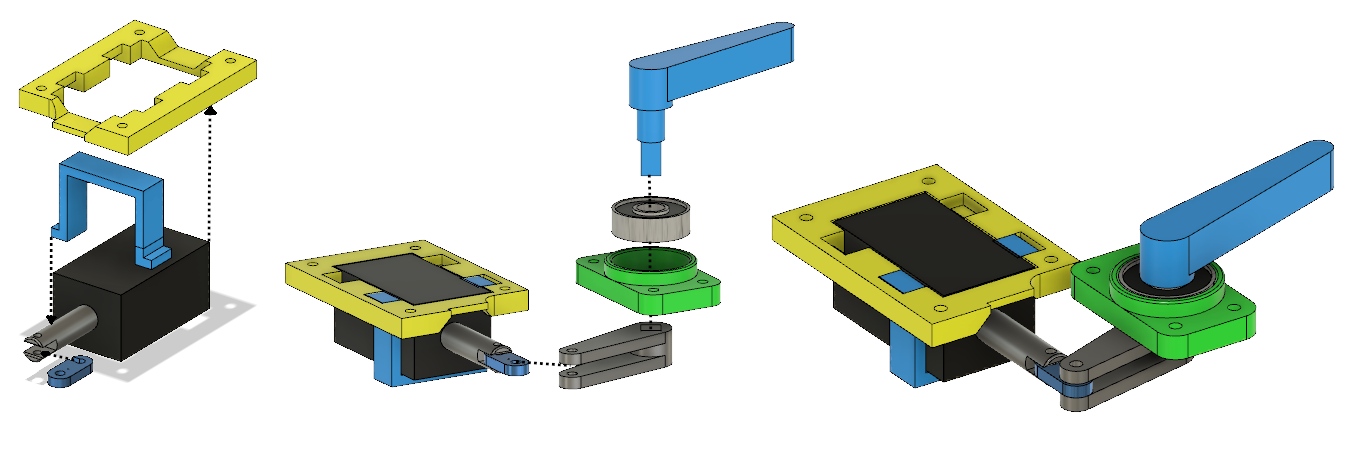
\includegraphics[width=\textwidth]{img/FlipperAssembly}
	\caption{Flipper assembly}
	\label{fig:flipperassembly}
\end{figure*}

\subsection{Pop Bumpers}
\subsubsection{Process and design}
Our first design for the pop bumpers was inspired by full sized pinball machines. It uses a linear solenoid for pulling a concave object, which when colliding with the ball, pushes it away. Most important is the detection mechanism, which uses a small plate that closes a circuit when pushed/moved. Examples of this can be seen in a video by Asker on YouTube \cite{asker_2017}. Although early tests showed that the plate was too complicated to work reliable.
Although as we improved the flipper mechanism, suddenly we had power to launch a steel ball. This meant that we could switch the pop bumpers to detect a circuit closed by the steel ball. Please see figure \ref{fig:newpop} for a image of this detection. Furthermore, for a view of the pop bumper with plate, refer to the "PopBumperWithSpoon" assembly in the "Pop Bumper" folder within the submitted Fusion 360 project.
\begin{figure}[H]
	\centering
	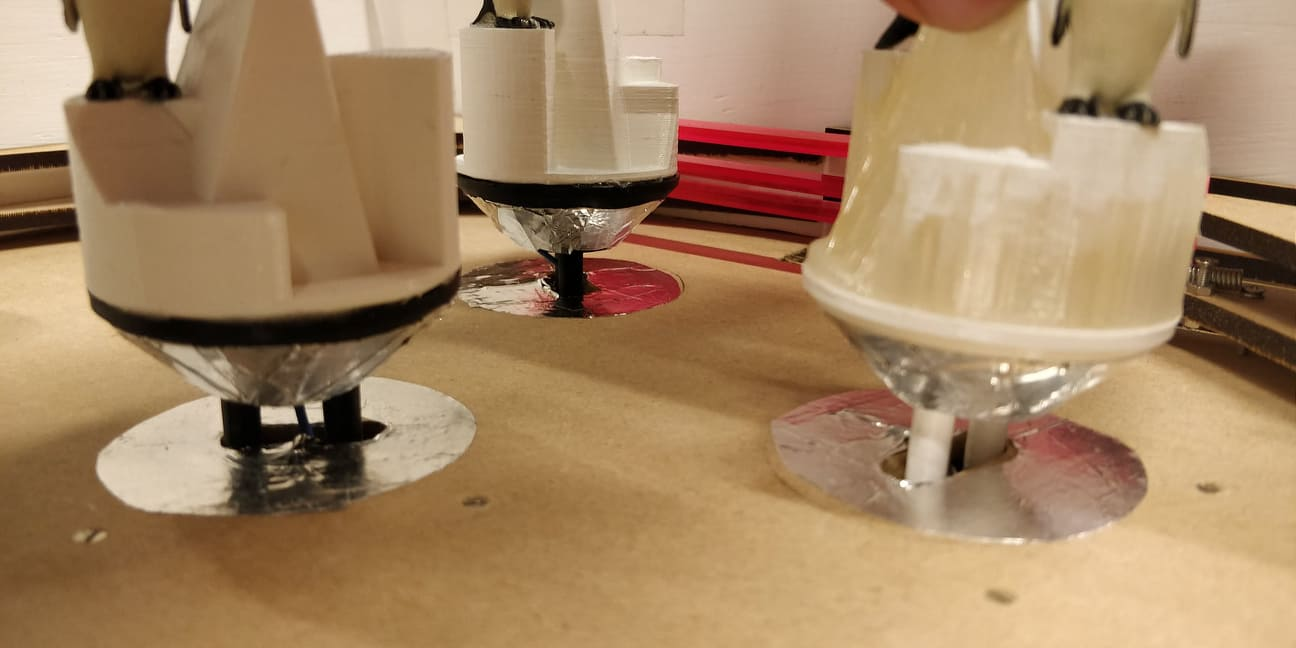
\includegraphics[scale=0.15]{img/new_bumper_design}
	\caption{The Final Pop Bumper Design}
	\label{fig:newpop}
\end{figure}

\subsubsection{Final Assembly}
The final pop bumper assembly is made up by a laser cut bracket which holds and limits the solenoid. The rest of the build is 3D printed, which includes a small bracket for the solenoid and a the hammer which pushes the ball away. Please see figure \ref{fig:bumperassembly} for an exploded view. Furthermore see Appendix \ref{appendix:cuts} for a overview of the cuts.
\begin{figure*}[h!]
	\centering
	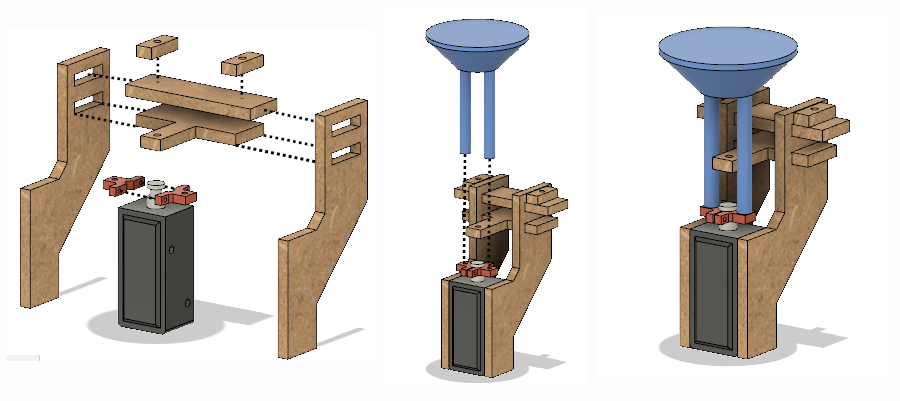
\includegraphics[width=\textwidth]{img/BumperAssembly}
	\caption{Pop Bumper Assembly}
	\label{fig:bumperassembly}
\end{figure*}

\subsection{Display}
For displaying the current score, a digital 7-segment display is used. 
It is milled into the backplate of the outer shell and encapsulated in a protective 3D-printed shell. 
Writing to the display is handled with a community Arduino library (\verb|DigitLedDisplay.h|) that talks to the  onboard MAX7219 chip. 

\subsection{Target switches}
\subsubsection{Process and design}
Switches are the main mechanism for our \textit{targets}. We found inspiration for the design of the targets in a YouTube video by \textit{Functional Design}\cite{functionaldesign_2017}. The concept builds on having a holder for a switch and a flap which is connected loosely to this holder such that it can be pushed in and activate the switch when the ball hits it. In order to visualise a hit we connected two LEDs to each holder, this means that whenever a switch is hit its associated LEDs will be turned on.

\subsubsection{Final Assembly}
The final target is modelled in Autodesk Fusion 360 and 3D printed afterwards. A target is composed of two switches, two holders, four LEDs, two flaps, and a 3D printed housing - the exploded view can be seen in figure \ref{fig:switchassembly}. We decided on having a target placed in each side of the board. The two targets share a board for their circuit which is then connected to the Arduino. When a switch is hit its associated LEDs are turned on and points are added to the total score. If a switch gets hit by the ball while the other switch on the target is turned on, all LEDs flashes for a short while and a bonus will be added to the score. 
\begin{figure*}
	\centering
	\includegraphics[width=\textwidth]{img/SwitchAssembly.png}
	\caption{Target Switch Assembly}
	\label{fig:switchassembly}
\end{figure*}

\subsection{Dividers and sensors}
\subsubsection{Process and design}
We wanted to add some mechanics to the top part of our board and we decided on having some \textit{dividers}, which should function as small walls. In order to register the ball we chose to add IR sensors in between these walls. The idea of the design of the walls is based on the fact that it had to hide a LED and a screw from the IR sensor.  

\subsubsection{Final Assembly}
Four 3D printed walls divide the top part of our board and three IR sensors are placed in each of the passages between these walls. Each wall contains an LED, and when a sensor registers the ball it will turn on the LED in the wall closest to it and points are added to the total score. If all three sensors are turned on at the same time, all LEDs will flash for a while and then turn off, also a bonus is added to the total score.
The sensors and the four LEDs share a board for their circuit and each component is connected to the Arduino. 

\subsection{Ball return mechanism}
The ball return mechanism consists of a slide going from a spring loaded pulley to a self-closing door on the playfield.

\subsubsection{Final assembly}
The parts are all laser cut using 4mm material of choice and then assembled using glue or screws. Exploded view is shown in figure \ref{fig:slideassembly}. Furthermore see Appendix \ref{appendix:cuts} for a overview of the cuts.
\begin{figure*}
	\centering
	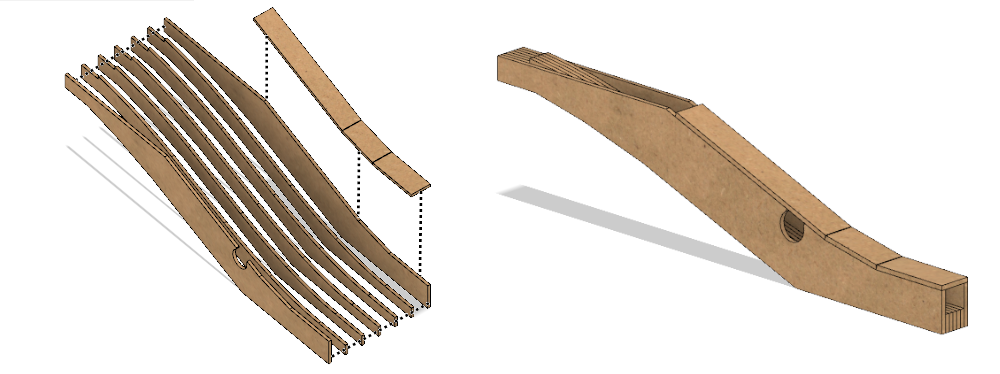
\includegraphics[width=\textwidth]{img/SlideMechanismAssembly}
	\caption{Slide mechanism assembly}
	\label{fig:slideassembly}
\end{figure*}

\subsection{The playfield}
The playfield of the machine is all bodywork on top, including the obstacles, ball return mechanism and bounding walls. All stationary walls were laser cut and fixed either by screws or brackets. The placement of the obstacles and point giving object can be changed and is not predetermined. Here, we give an example of how to place these.

\subsubsection{Final assembly of bodywork}
Every wall piece is laser cut from a 4mm material of choice. Then they are mounted with screws and spacers. Please see figure \ref{fig:bodyassembly} for an exploded view. Furthermore see Appendix \ref{appendix:cuts} for a overview of the cuts.
\begin{figure*}
	\centering
	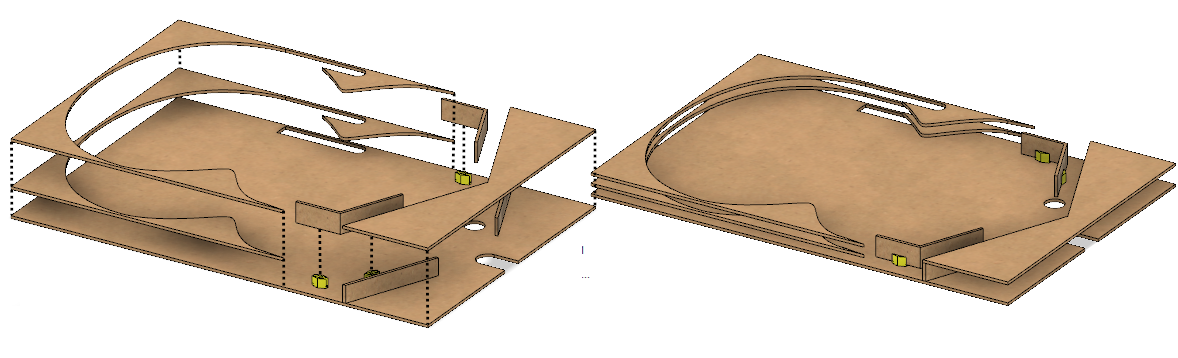
\includegraphics[width=\textwidth]{img/PlayFieldBodyAssembly}
	\caption{Playfield bodywork assembly}
	\label{fig:bodyassembly}
\end{figure*}

\subsubsection{Attaching the mechanisms to playfield}
Flippers and the ball-return mechanism both fit into the appropriate holes. All the other mechanism have appropriate holes for screws, and these can be attached whereever on	es sees fit. Please see figure \ref{fig:mechanismassembly} for an exploded view.
\begin{figure*}
	\centering
	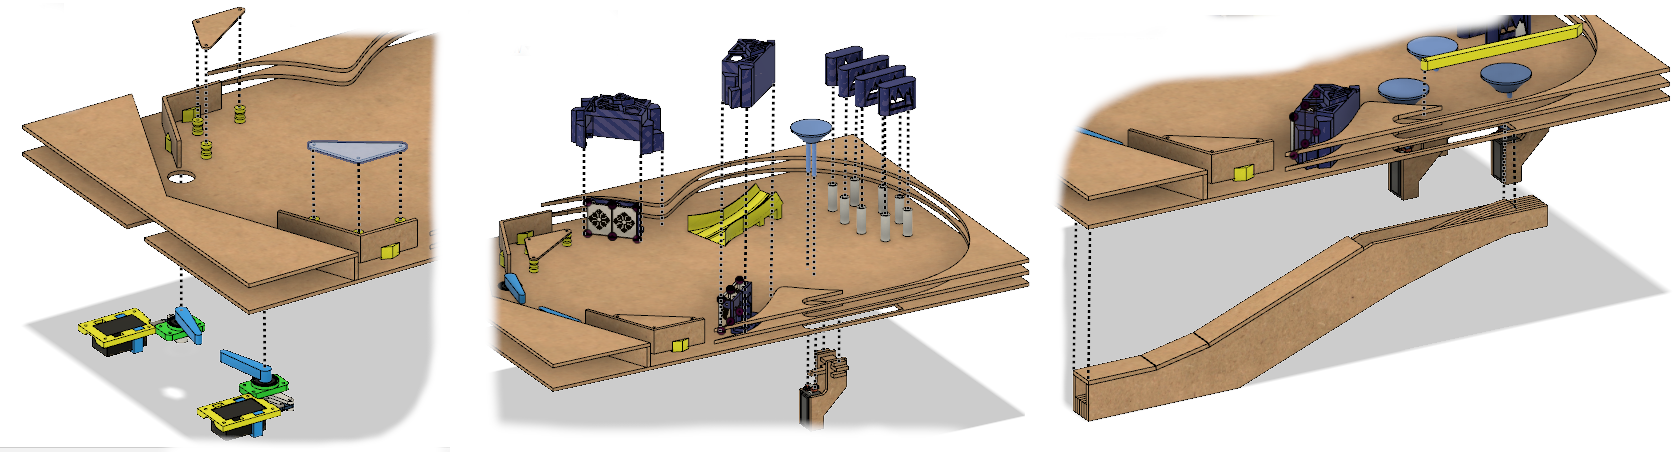
\includegraphics[width=\textwidth]{img/PlayFieldMechanismAssembly}
	\caption{Assembly for all mechanisms on playfield.}
	\label{fig:mechanismassembly}
\end{figure*}

\subsection{The Software Implementation}
The whole show is driven by an Arduino Mega, for which a wiring diagram is supplied in figure \ref{fig:wiring}.
Black wires indicate input, {\color{red} red} wires indicate output, and {\color{blue} blue} are for two-way communication. 
An more comprehensive overview of the functional blocks in the machine is given in appendix figure \ref{fig:funcdiag}

The pinball machine domain is largely event-driven, unlike the sequential nature of the Arduino. 
We had to avoid use of the delay function in order to be responsive to button/switch/IR sensor inputs at arbitrary times. 
A concurrent model, inspired by the Adafruit guide in \cite{multitasking_arduino}, was chosen as the solution. We describe this model in more detail in appendix \ref{appendix:programming model}.
\begin{figure}[h]
	\centering
	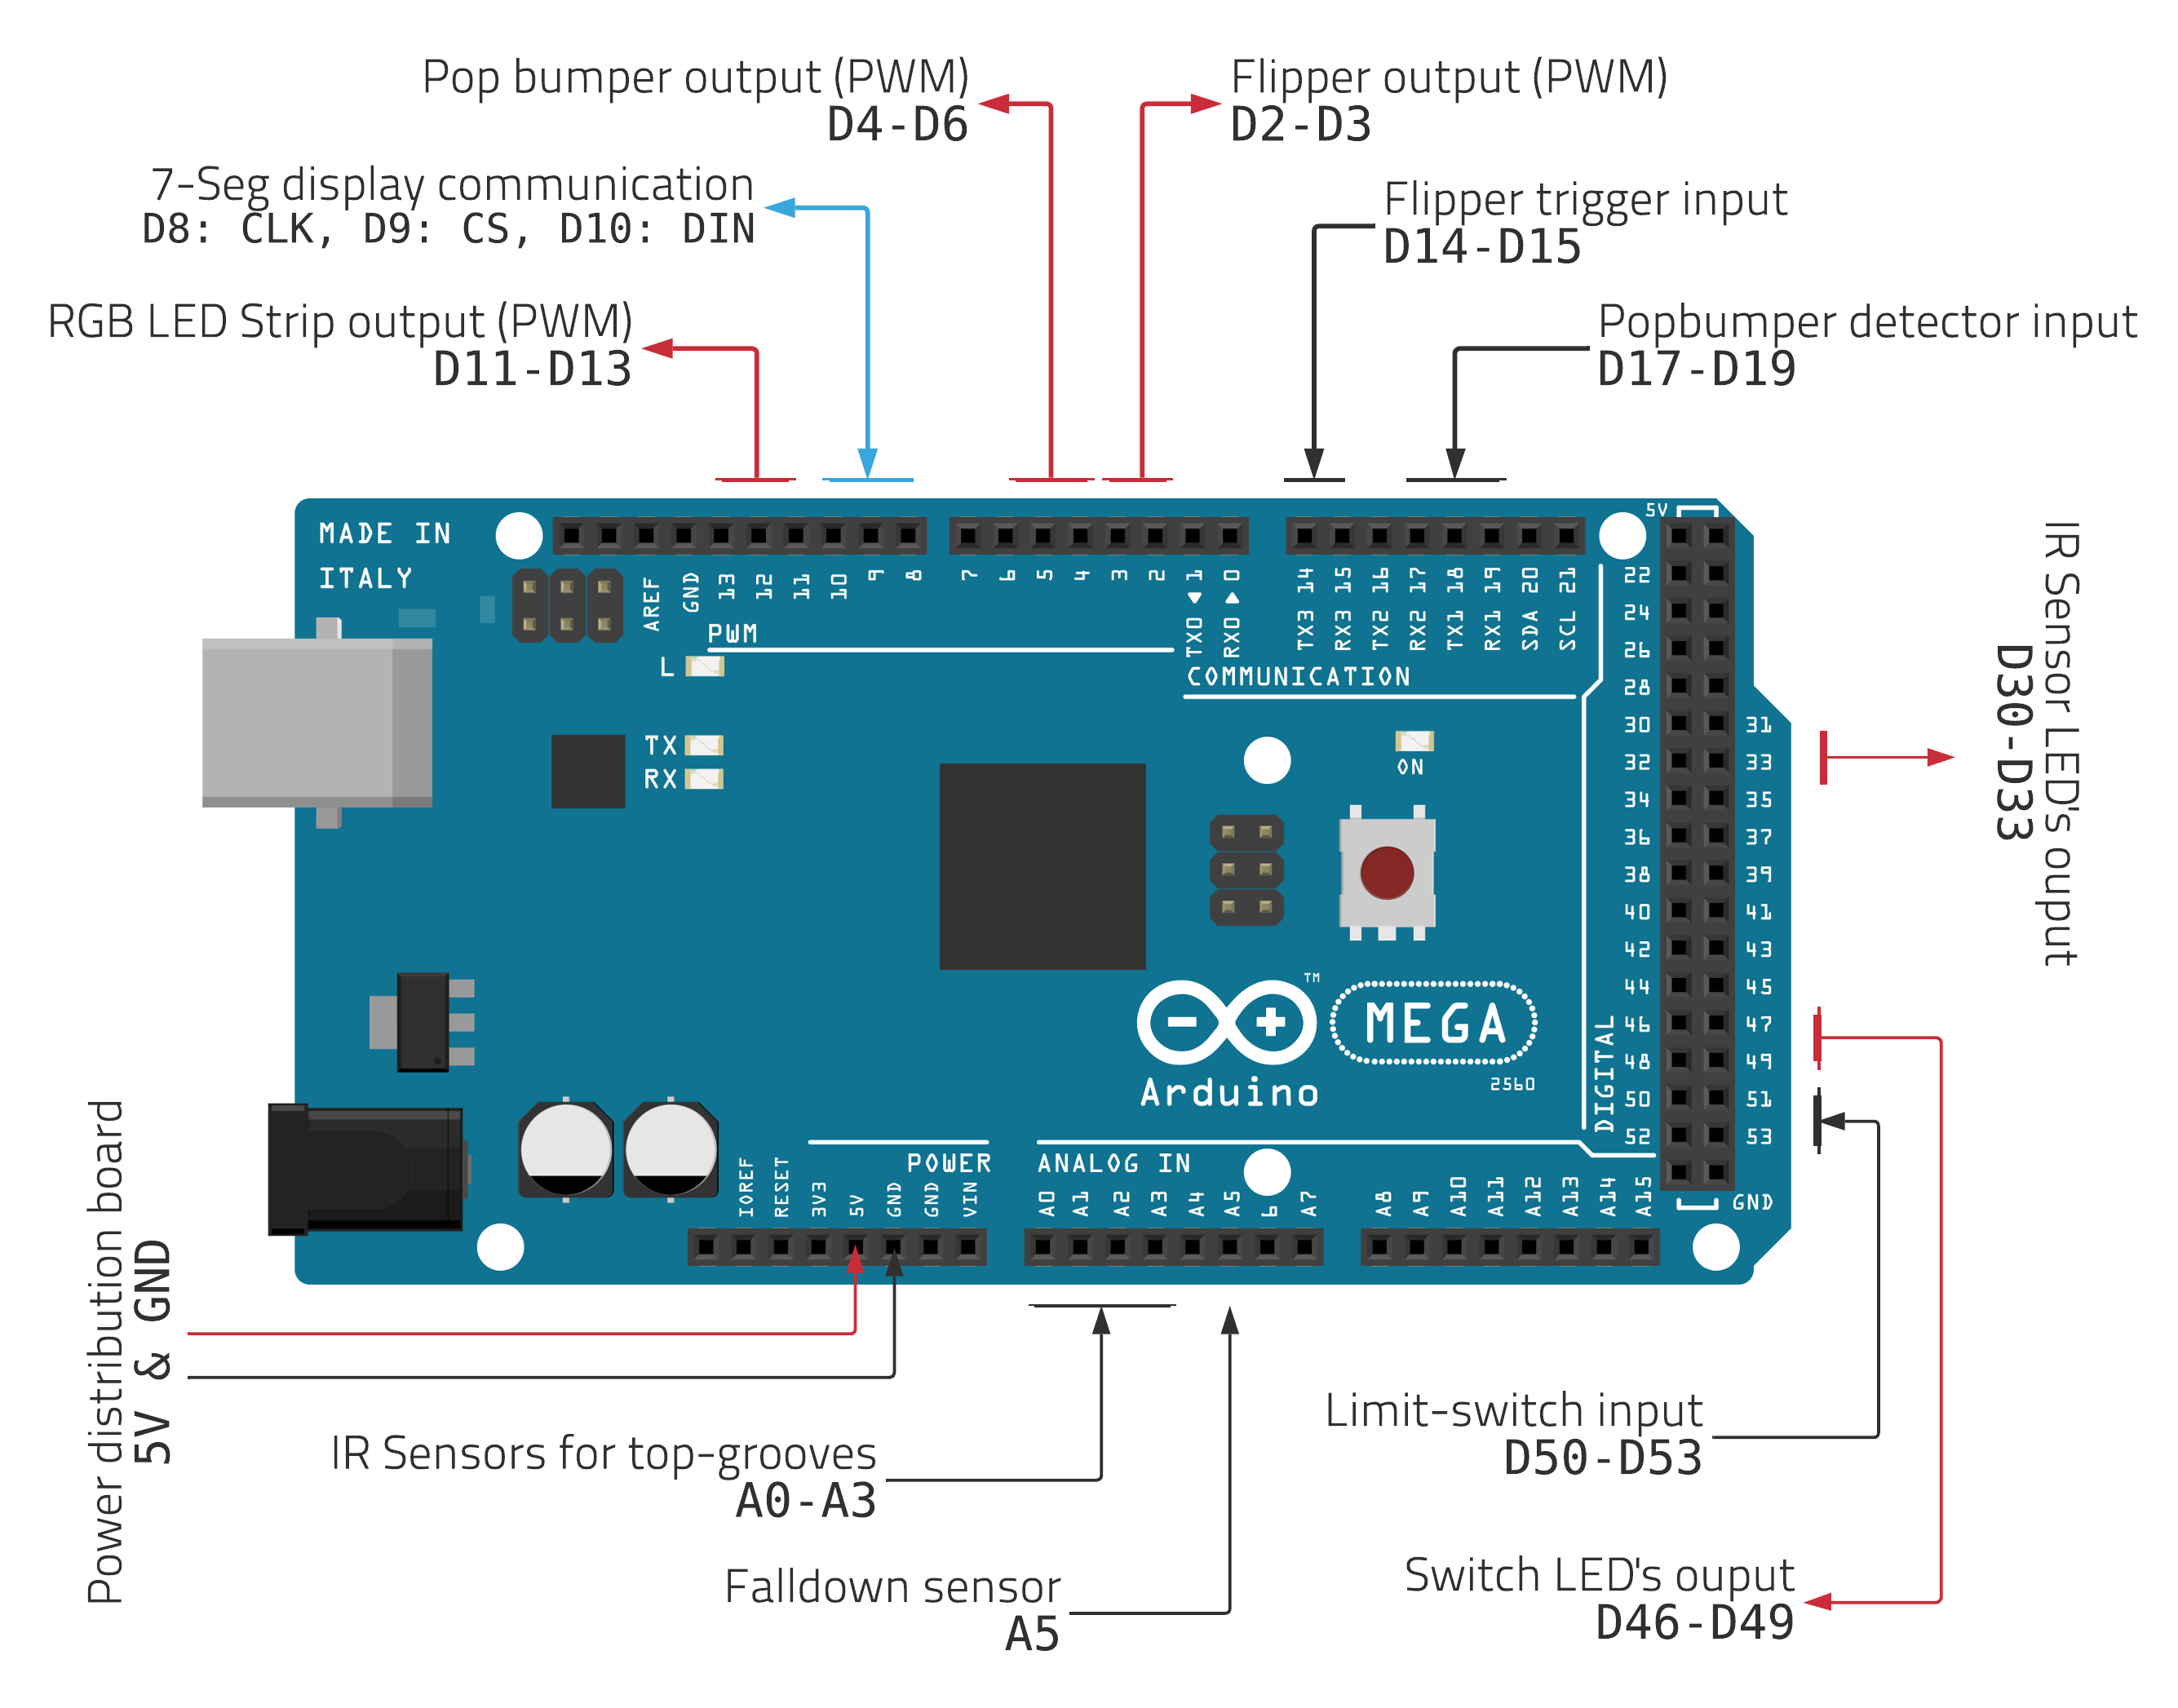
\includegraphics[width=0.46\textwidth]{wiring_diagram}
	\caption{How the Arduino Mega is wired up to the project interface boards.}
	\label{fig:wiring}
\end{figure}
\subsection{Putting it all together}
\begin{figure}[h]
	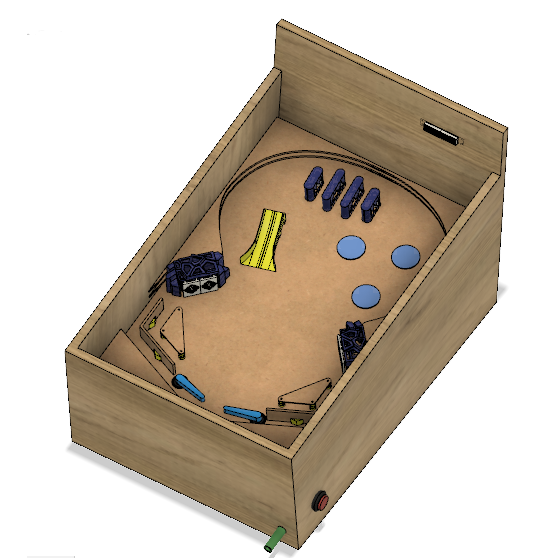
\includegraphics[width=\textwidth/2]{FinalAssembly}
	\caption{View of the final assembly 3D reference.}
	\label{fig:finalassembly}
\end{figure} 
The final playfield assembly is lowered into a plywood box with cut rails for support. Here, the segment display and spring loaded mechanism is attached. Figure \ref{fig:finalassembly} shows the final assembled version 3D reference model. This model, named FinalAssembly in Fusion 360, can be used to source the necessary dimensions of the surrounding box.


